\chapter{RELATED WORK}
\label{related}
% 1-2 pghs describing whats in this chapter.

\section{Software Defined Networking}
\label{related:sdn}
SDN provides a networking device model where the control and data planes are decoupled from one another, where a single control plane is responsible for distributing application execution across a set of network switches viewed as a unified data plane instance. Applications generally operate at the control plane level and rely on distributed platforms, such as OpenVSwitch (OVS) \ref{ovs}, to push the logic down to the hardware level. Generally a hypervisor sits on top of each switch and helps orchestrate the entire system.d


\section{Networking Applications}
\label{related:apps}
Not all networking applications operate in the same conceptual space, that is, they generally act as a part of a larger system. Applications can operate on a particular traffic flow, a node within a network, or across the entire network.
% Add more to this.

\section{OpenFlow}
\label{related:of}
% Add more to this.
The OpenFlow model defines a messaging layer that the control and, potentially distributed, data plane(s) can communicate through. This is embodied in the OpenFlow Protocol, which specifies a set of ``instructions'' that the control and data planes must support. 

\section{DPDK}
\label{related:dpdk}
Describe DPDK.

\section{Open Data Plane}
\label{related:odp}
Talk about this a little bit.

\section{OpenVSwitch}
\label{related:ovs}
Emphasize how open vswitch works to distibute sdn apps.
\begin{figure}[h]
\centering
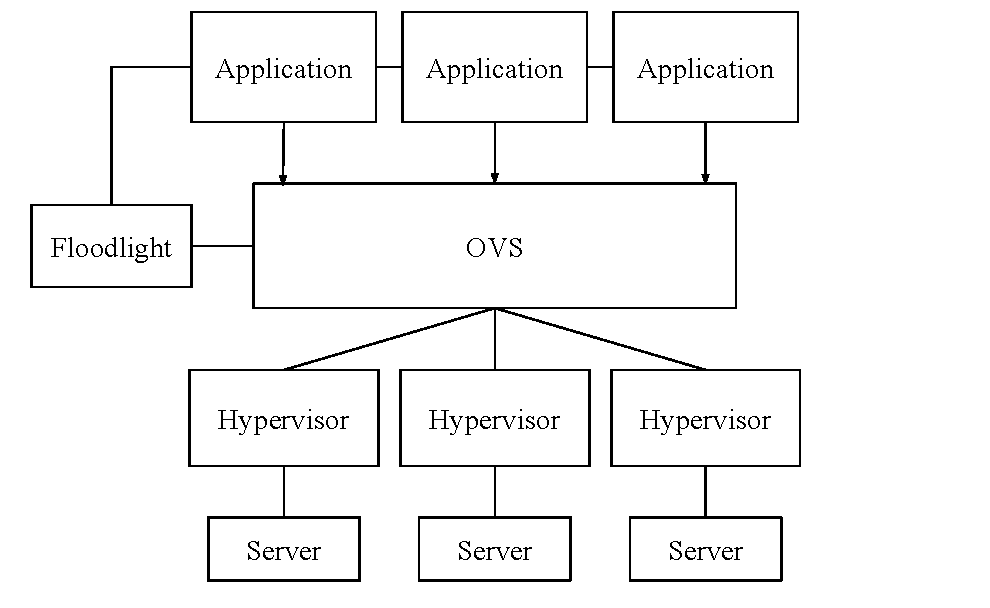
\includegraphics[scale=0.5]{ovs_arch}
\caption{The OpenVSwitch architecture.}
\label{related:ovs_arch}
\end{figure}

\section{NetASM}
\label{related:netasm}
Talk, at length, about netasm. Can bring up riscv here too.

\subsection{RISC V}
% Rewrite this.
Our next approach focused more on the interaction between the language and
runtime components of our system, with the hopes of being able to execute
the language in a native ISA. We came across an extensible ISA, RISC V, that
provided not only basic arithmetic, logical, and control flow instructions but
also left room for a number of custom instructions. This seemed like a great
way to incorporate specialized network programming instructions into a native
format. Unfortionately, this would also require that we interpret and implement
all of the supported instructions in the set in an virtual machine. As a result
the execution took a serious hit in terms of performance at the cost of this
flexibility. This project requires a fine balance of flexibility and
performance, and the deviation between these properties was too great.

\section{Heterogenous Compute Platforms}
\label{related:hcp}
Discuss the heterogenous compute models considered.

\subsection{HSAIL}
\label{related:hcp:hsail}
Heterogenous System Architecture Intermediate Langauge.

\subsection{OpenCL}
\label{related:hcp:ocl}
Open Compute Language.

\subsection{CUDA}
\label{related:hcp:cuda}
Compute Unified Device Architecture.

\section{Frameworks}
\label{related:frameworks}
Discuss the frameworks considered.

\subsection{Seastar}
\label{related:frameworks:seastar}
Bad ass, if you've got the HW to support it.

\subsection{Libevent}
\label{related:frameworks:libevent}
Very complicated, not easy to target custom backends (dpdk).
